\documentclass[reprint,english,notitlepage]{revtex4-2}
\usepackage{amsmath}
\usepackage[mathletters]{ucs}
\usepackage[utf8x]{inputenc}
\usepackage[english]{babel}
\usepackage{esint}
\usepackage{physics,amssymb}
\usepackage{graphicx}
\usepackage{xcolor}
\usepackage{hyperref}
\usepackage{listings}
\usepackage{subfigure}
% \usepackage[style=science, backend=biber]{biblatex}
% \addbibresource{Report_Part_5.bib} TODO: Slett før innlevering
\hypersetup{
    colorlinks,
    linkcolor={red!50!black},
    citecolor={blue!50!black},
    urlcolor={blue!80!black}}

\lstset{inputpath=,
    backgroundcolor=\color{white!88!black},
    basicstyle={\ttfamily\scriptsize},
    commentstyle=\color{magenta},
    language=Python,
    morekeywords={True,False},
    tabsize=4,
    stringstyle=\color{green!55!black},
    frame=single,
    keywordstyle=\color{blue},
    showstringspaces=false,
    columns=fullflexible,
    keepspaces=true}

\begin{document}

\title{Satellite Launch}
\author{Oskar Idland \& Jannik Eschler}
\date{\today}
\affiliation{Institute of Theoretical Astrophysics, University of Oslo}

\begin{abstract}
    This is an abstract \colorbox{red}{Complete this summary at the end of the paper}
\end{abstract}
\maketitle

\section{Introduction} \label{sec:introduction}
The purpose of this project is the launch of our shuttle.
Interplanetary travel have huge cost and risks.
Therefore, we must guarantee success by planning ahead of our journey.
We will develop a simulation to visualize our orbit given some parameters as a means to get a good picture of where we will end up.\\

After completing these final preparations and simulations, we will then send our spacecraft towards its destination.
The launch and interplanetary travel will be executed based on the calculations and simulations we have done in the previous parts of this series of reports.
However, as we have done some assumptions and simplifications in our simulations, we expect some deviations in the actual path of the spacecraft.
This is due to factors such as solar winds, gravitational forces from small objects and friction.\\
To reach our destination, we will therefore launch the rocket on the simulated trajectory and do some corrections of our trajectory, if the actual trajectory deviates from the simulated trajectory.\\
These corrections will be done by firing our rocket engine to change our velocity, and therefore our trajectory as described in figure~\ref{fig:boost_fig}.

\begin{figure}[h]
    %% H(Here), h(here approx), t(top of page), b(bottom of page)
    \centering
    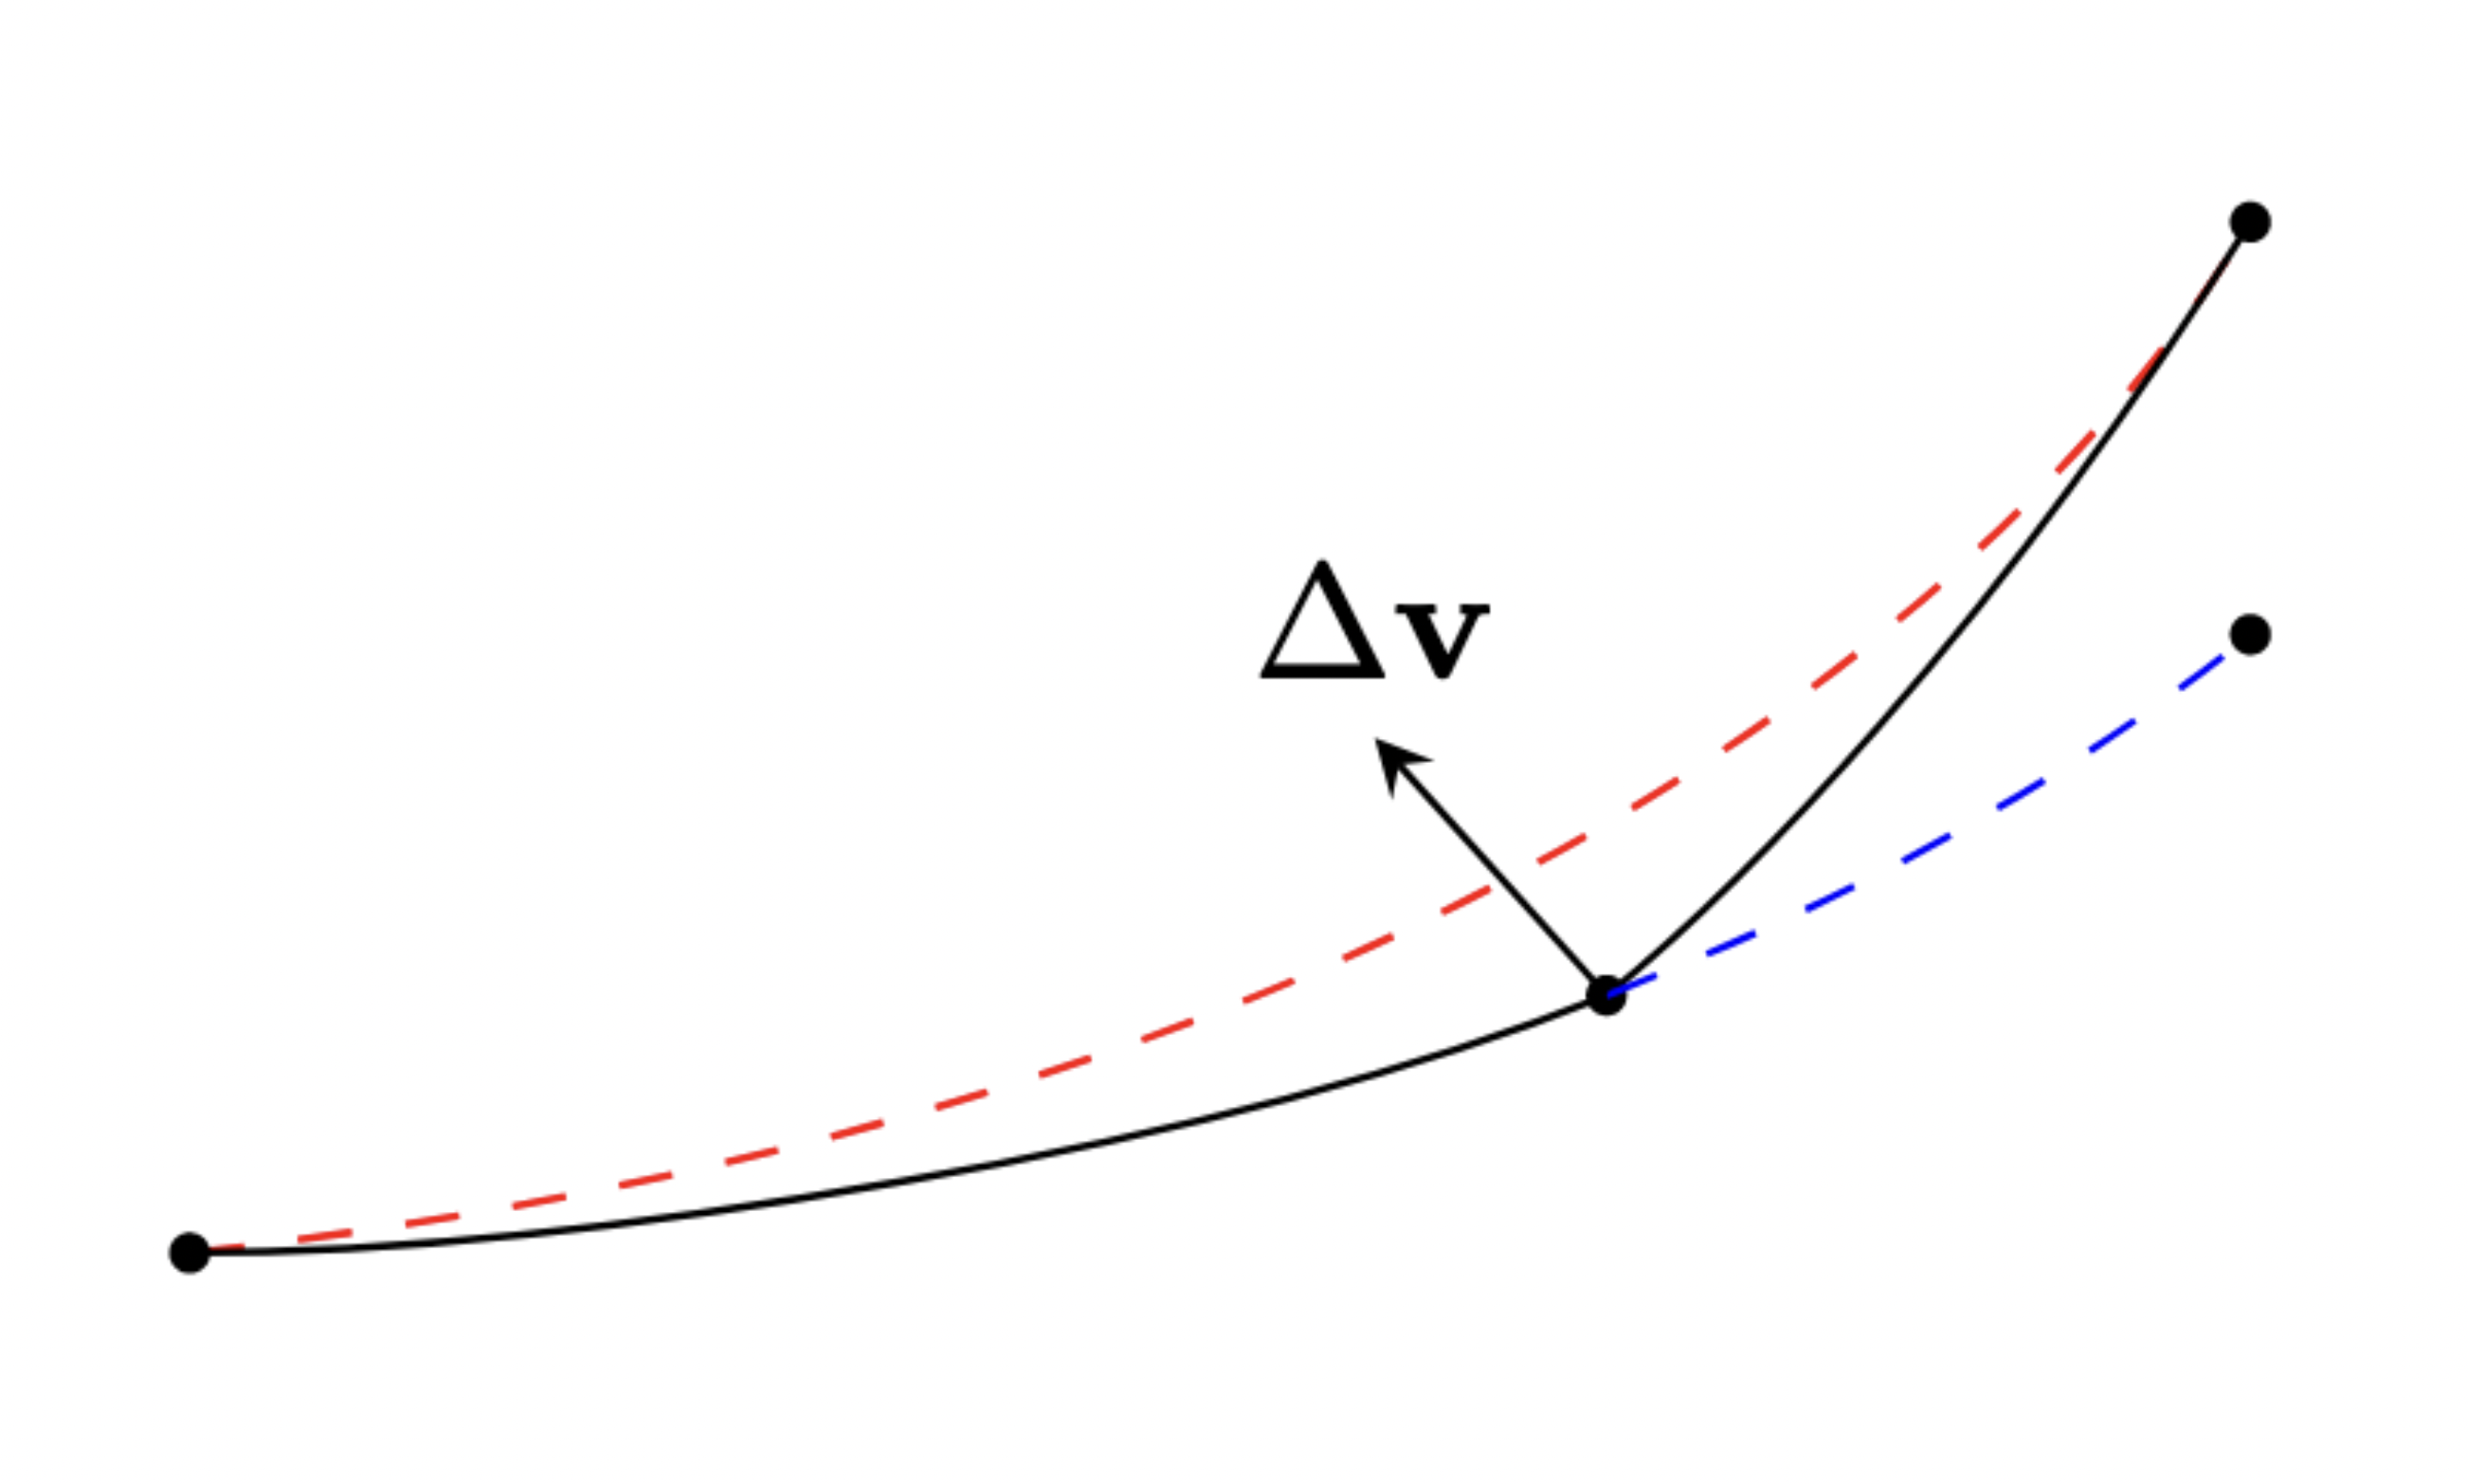
\includegraphics[scale=0.12]{Figures/boost_fig}
    \caption{Visualisation of a correctional boost to change the trajectory. The actual trajectory (black) deviates from the planned trajectory (red), then a trajectory
        correction $\Delta v$ is used to prevent the trajectory from drifting further away (blue). From %~\parencite[][]{project_description5} TODO: Remove Comment
    }\label{fig:boost_fig}
\end{figure}

The goal is to get close enough to the planet so that the gravitational forces from the planet dominate over the gravitational forces from the rest of the planets and the star.
We can then initialise an orbit injection manoeuvre to enter the orbit around the planet.\\

When in orbit around the destination planet, we will have to orient ourselves and analyze the orbit we are in.
Using the onboard instruments we will determine all necessary parameters to be able to fully simulate the orbit.
This is to predict the movement and position of our spacecraft at a later point in time, which will be necessary to determine a time and position for the landing of our rover.
Furthermore, we can determine the stability of the orbit based on its shape.
The more eccentric an orbit is, the more unstable it is.



\section{Theory} \label{sec: theory}
A description of the Leapfrog simulation method can be found in section II of the second paper %~\parencite[][]{part2} TODO: Delete Comment.
of this series of papers


\section{Method} \label{sec: method}
\subsection{Simulating trajectory} \label{ssec: simulating trajectory}
To simulate the trajectory our shuttle will have we simplify our system into a N-body system where all the planets and star will be combined into a single body.
As the mass of the shuttle is so small in comparison to the rest of our solar system, we will disregard its gravitational pull.
First we will calculate the center of mass $ \mathbf{CM} $
\[
\mathbf{CM} = \frac{1}{M} \sum_{i} m_i \mathbf{r_i}
\]
where $ M $ is the total mass of our solar system and $ m_i $ and $ r_i $ is the mass and position of each planet respectively.
We then find the total momentum $ \mathbf{p} $ as a sum of all the momentum of each planet in the system
\[
\mathbf{p} = \sum_{i} m_i \mathbf{v_i}
\]
where $ \mathbf{v_i} $ is the velocity of each planet. 
As we use the position of the star as origin we represent the position of the $ \mathbf{CM} $ as $ \mathbf{r}_{sys} $.
This position changes over time with a velocity $ \mathbf{v}_{sys} = \frac{\mathbf{p}}{M} $.
As the shuttle travels, its position $ \mathbf{r} $ will be influenced by its initial velocity $ \mathbf{v_0} $ and the gravitational pull of the system.
The acceleration of the spacecraft is given by
\[
\mathbf{a} = -G \frac{M}{\left\vert \mathbf{r} - \mathbf{r}_{sys} \right\vert ^{3}} \left( \mathbf{r} - \mathbf{r}_{sys} \right)
\]

Using the leapfrog method for numerical integration we can calculate the full trajectory of our shuttle.
\newline


\subsection{Getting close enough to the target planet}\label{subsec:getting-close-enough}
To make our journey as easy as possible we first try to check where our home planet and target planet are the closest.
Using the orbits calculated from the second paper %~\parencite[][]{part2} TODO: Delete comment
of this series of papers we iterate over all positions and check at which time $ t_{0} $ the distance is the smallest.
\colorbox{red}{Legg til figur av hvor planetene er nærmest her eller i } \colorbox{red}{resultat??}.
With this position it seems favorable to launch from the bottom of our planet $ \mathbf{r}_0 $.
To figure out the direction to launch our planet we begin by using an educated guess by pointing the shuttle directly at the target planet.
We then continue by simulating the orbit for multiple, evenly spaced out angles from the angle of the vector pointing directly at the target planet $ \mathbf{v}_0 $, to a max angle of $ \pi/8 $ radians just to get a picture of how the launch will look for different angles.
Now we have a wide span of possible angles.
Before narrowing the angles down we will iterate over possible values for $ \left\vert \mathbf{v}_0 \right\vert  $.
This gives us an idea of how fast the shuttle needs to travel for it to get even close to reaching the target planet.
Once this is done, we will iterate over a range of angles and velocities, find the time we are the closest to the target planet and the distance.
For each case we will check if the smallest distance $ d $ satisfy the requirement for beginning orbit around target planet given by
\[
d \le l, \qquad l = \left\vert \mathbf{r} \right\vert \sqrt{\frac{M_{target}}{M_{star}}}  
\]




\subsection{Launching the Spacecraft}\label{subsec:launching-the-spacecraft}
    Having simulated the necessary parts of the launch, journey and conditions on our destination planet, we can now send the spacecraft on its journey.\\
    As stated in section~\ref{sec:introduction}, the time and direction of the launch will be based on our simulations.
    We will therefore launch the rocket at the point in time, which was deemed preferable in our simulations.\\

    After reaching space, the spacecraft will orient itself, and perform an initial boost to enter the simulated trajectory.
    To execute such a correctional boost, the onboard computer first calculates the required change in velocity.
    Thereafter, we use the onboard gyroscopic stabilizer to rotate the spacecraft.\\
    Since all forces acting on the spacecraft when it is coasting in space are conservative, the angular momentum must be conserved.
    The gyroscopic stabilizer uses three inertial wheels, which can be accelerated using electric motors to induce an angular momentum to the rocket due to the conservation of the total angular momentum.
    This means, we can rotate the rocket without using any fuel.\\
    After rotating the rocket, the main rocket engine will perform a short boost to change the velocity to the velocity required to enter the simulated trajectory.
    The exact duration of the boost, and therefore the change of velocity $\Delta \textbf{v}$ has been determined by the onboard computer.
    As we have measured the position $ \textbf{s}$ and velocity $\textbf{v}$ of the spacecraft when orienting ourselves after the launch, we can determine the required velocity $ \textbf{v}_{req}$ at the current position to enter a trajectory leading to the destination planet, using the method described in section~\ref{ssec: simulating trajectory} and~\ref{subsec:getting-close-enough}.
    The required change in velocity can then easily be found by subtracting.

    \begin{align*}
        \Delta\textbf{v} = \textbf{v}_{req} - \textbf{v}
    \end{align*}

    However, this only gives us a vector.
    To find the direction and magnitude of the boost, we use some trigonometry.
    \begin{align*}
        \Delta\textbf{v} = [\Delta v_x, \Delta v_y]\\
        |\textbf{v}| = \sqrt{{\Delta v_x}^2 + {\Delta v_y}^2}\\
        \theta = \arctan \left(\frac{\Delta v_y}{\Delta v_x}\right)
    \end{align*}

    We then use the calculations from the first paper %~\parencite[][]{part1} TODO: Delete comment
    of this series of papers to calculate the amount of fuel used for a given $|\Delta\textbf{v}|$ in the process of the correction maneuver

    Since the duration of the calculations, rotation of the rocket and boost are insignificant compared to the duration of the journey to the destination planet, we will regard them as instantly.
    A representation of such a boost can be seen in figure~\ref{fig:boost_fig}.\\

    After the initial orientation and boost, the spacecraft will be departing on the planned trajectory to the destination planet.
    However, due to inaccuracies in the simulations, gravitational forces from small objects and solar winds, the actual trajectory of the spacecraft will deviate from the simulated trajectory.
    We will therefore orient the spacecraft at regular intervals and compare the position and velocity to the simulated trajectory.
    If the deviation is gets too large, we will initiate a correctional boost.
    This boost will be executed in exactly the same way as the initial boost after the launch of the spacecraft.\\

    The limit of the deviation, when we decide to initiate a boost needs to be chosen carefully as correctional boosts for smaller deviations require less fuel, but may need to happen more often.
    As we only have a limited amount of excess fuel after the launch, we need to be careful to be as efficient as possible when making corrections to our trajectory.\\
    This process of coasting on a trajectory, and correctional boosts will then be repeated until we arrive at the destination planet.

    The trajectory of the spacecraft will then end when we are within the required distance $l$ from the planet as calculated in section~\ref{subsec:getting-close-enough} and the velocity of the spacecraft relative to the planet only has a tangential component.
    In other words, if equation~\eqref{formula1} holds.
    \begin{align}
        \textbf{v}(t) \cdot \textbf{s}(t) = 0 \label{formula1}
    \end{align}
    At this point we have to perform another correctional boost in the opposite direction than our velocity to slow the spacecraft and enter into an orbit around the planet.
    The change of velocity $\Delta \textbf{v}$ depends on the velocity of the spacecraft before the boost, and the distance of the spacecraft to the center of the planet.\\
    The velocity $\textbf{v}_{tan}$ needed to be in a perfectly circular orbit can be calculated using the formula for the centripetal acceleration and the formula for gravitational acceleration.
    \begin{align*}
        a_c &= G \frac{M_{Planet}}{r^2}\\
        a_c &= \frac{\textbf{v}_{tan}^2}{r}\\
        \textbf{v}_{tan}^2 &= G \frac{M_{Planet}}{r}\\
        \textbf{v}_{tan} &= \sqrt{G \frac{M_{Planet}}{r}}
    \end{align*}
    Since both $ \textbf{v}$ and $\textbf{v}_{tan}$ are tangential velocities and therefore point in the same direction, we can now simply determine the required change in velocity $\Delta \textbf{v}$ by subtracting.
    \begin{align*}
        \Delta \textbf{v} = \textbf{v} - \textbf{v}_{tan}
    \end{align*}

    After this burn, the velocity of the spacecraft matches the velocity required to be in a perfectly circular orbit around the planet.
    The radius of the orbit has been measured and will remain constant.
    To determine the orbital period, we can use Kepler's third law of planetary motion~\eqref{Kepler3}.
    \begin{align}
        \frac{a^3}{T^2} = C \label{Kepler3}
    \end{align}




\section{Results} \label{sec: results}

\section{Discussion} \label{sec: discussion}

\section{Conclusion} \label{sec: conclusion}

\section{Appendix} \label{sec: appendix}

\section*{ACKNOWLEDGMENTS}

\newpage
% \printbibliography TODO: Remove Comment
\end{document}